\documentclass[12pt]{article}

\usepackage{fullpage}
\usepackage{fancybox}
\usepackage{graphicx}
\usepackage{amssymb}
\usepackage{amsmath}
\usepackage{enumerate}
\usepackage{float} 
\usepackage{multirow}


%%%%%%%%%%%%%% Capsule %%%%%%%%%%%%%%%%%%%%%%%%%%%%%%%%%%%%%%%%%%%
\newcommand{\capsule}[2]{\vspace{0.5em}
  \shadowbox{%
    \begin{minipage}{.90\linewidth}%
      \textbf{#1:}~#2%
    \end{minipage}}
  \vspace{0.5em} }
%%%%%%%%%%%%%%%%%%%%%%%%%%%%%%%%%%%%%%%%%%%%%%%%%%%%%%%%%%%%%%%%%%

\newcounter{ques}
\newenvironment{question}{\stepcounter{ques}{\noindent\bf Question \arabic{ques}:}}{\vspace{5mm}}

\begin{document} 

\begin{center} \Large\bf
COMP 4107: Neural Networks -- Assignment 2\\
-- Winter 2026 -- 
\end{center} 

\begin{center}
{\bf Due:} February 13th, 2026 \\
Group 51 \\
Andrew Wallace - 101210291\\
Christer Henrysson - 101260693\\
Amr Altaweel - 101276934\\[1em]
\end{center}

\newpage 

\section*{Question 1}
Please see \texttt{assignment2.py} for implementation.
\section*{Question 2}
Please see \texttt{assignment2.py} for implementation.
\section*{Question 3}
Please see \texttt{assignment2.py} for implementation.
\section*{Question 4}
Please see \texttt{assignment2.py} for the full implementation. \\
The following plots were generated for the below experiments. Note that the data was split into 70\% training data, 15\% validation data, and 15\% test data for all experiments.
\begin{enumerate}[(a)]
  \item Number of neurons in each hidden layer
  \begin{figure}[H]
    \centering
    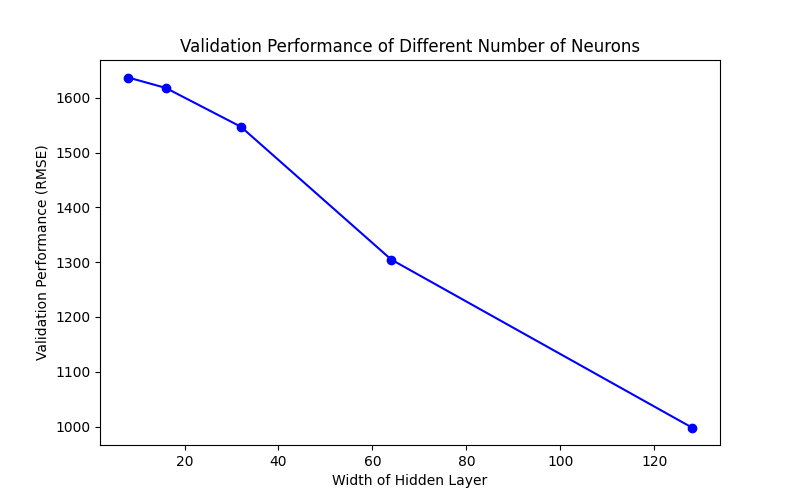
\includegraphics[width=0.7\textwidth]{neurons.png}
    \caption{Neurons Experiments}
    \label{fig:n_plot}
  \end{figure}
  \item Number of hidden layers in the network 
  \begin{figure}[H]
    \centering
    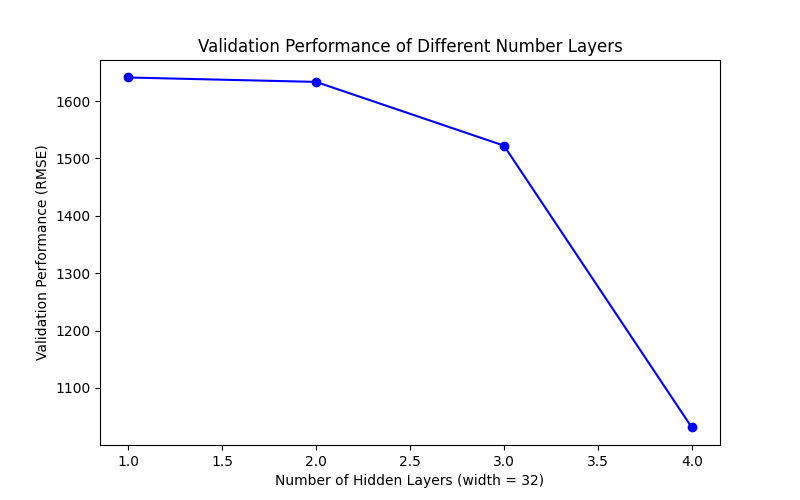
\includegraphics[width=0.7\textwidth]{layers.png}
    \caption{Layers Experiments}
    \label{fig:l_plot}
  \end{figure}
  \item Number of epochs used for training
  \begin{figure}[H]
    \centering
    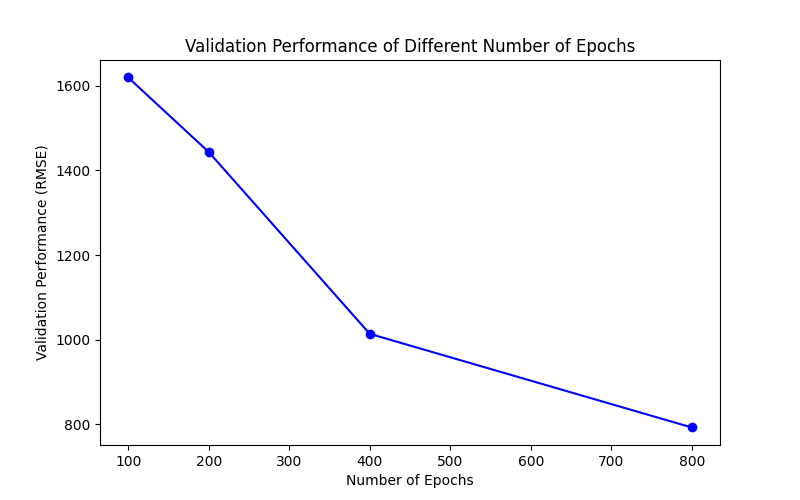
\includegraphics[width=0.7\textwidth]{epochs.png}
    \caption{Epochs Experiments}
    \label{fig:ep_plot}
  \end{figure}
  \item Different activation functions
  \begin{figure}[H]
    \centering
    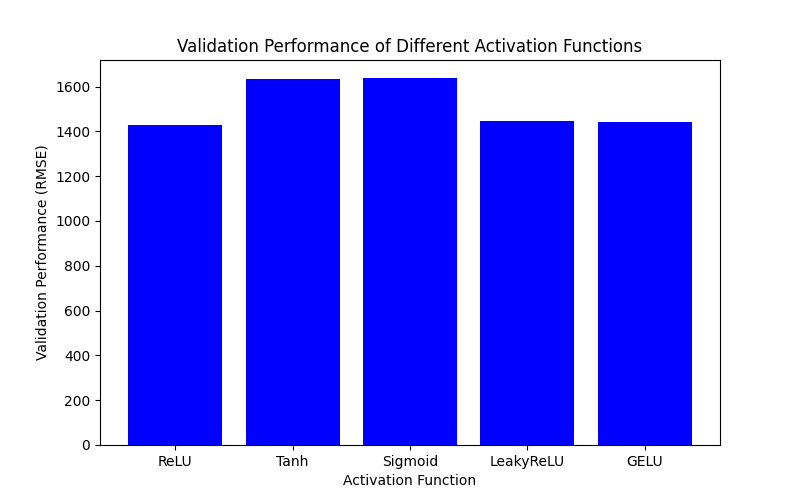
\includegraphics[width=0.7\textwidth]{activations.png}
    \caption{Activation Function Experiments}
    \label{fig:af_plot}
  \end{figure}
  \item Model with the best performance \\
  The best single performing model out of all experiments was the epoch model in part (b) that used 800 epochs. The performance on the training, validation, and test set is given below.\\[1em]
  Best Model Performance (single model from experiments): epochs = 800
  \begin{itemize}
    \item Train RMSE: 744.9811401367188
    \item Validation RMSE: 822.7666625976562
    \item Test RMSE: 800.5404052734375
  \end{itemize}
  The best overall performing model when combining the models from each experiment was the following model. \\
  Best Overall Model Performance (combining models from experiments):
  \begin{itemize}
    \item Neurons: 128
    \item Layers: 3 layers, each with width = 32 ([32, 32, 32])
    \item Epochs: 800
    \item Activation Function: ReLU()
  \end{itemize}
  The performance on the training, validation, and test set is given below.
  \begin{itemize}
    \item Train RMSE: 616.2930297851562
    \item Validation RMSE: 639.0341796875
    \item Test RMSE: 704.6664428710938
  \end{itemize}
  We can see that combining the best models from each experiment yields a lower RMSE compared to the single model.

\end{enumerate}

\end{document} 
